\documentclass[journal,12pt,twocolumn]{IEEEtran}
\usepackage{setspace}
\usepackage{gensymb}
\usepackage{caption}
%\usepackage{multirow}
%\usepackage{multicolumn}
%\usepackage{subcaption}
%\doublespacing
\singlespacing
\usepackage{csvsimple}
\usepackage{amsmath}
\usepackage{multicol}
%\usepackage{enumerate}
\usepackage{amssymb}
%\usepackage{graphicx}
\usepackage{newfloat}
%\usepackage{syntax}
\usepackage{listings}
\usepackage{iithtlc}
\usepackage{color}
\usepackage{tikz}
\usetikzlibrary{shapes,arrows}



%\usepackage{graphicx}
%\usepackage{amssymb}
%\usepackage{relsize}
%\usepackage[cmex10]{amsmath}
%\usepackage{mathtools}
%\usepackage{amsthm}
%\interdisplaylinepenalty=2500
%\savesymbol{iint}
%\usepackage{txfonts}
%\restoresymbol{TXF}{iint}
%\usepackage{wasysym}
\usepackage{amsthm}
\usepackage{mathrsfs}
\usepackage{txfonts}
\usepackage{stfloats}
\usepackage{cite}
\usepackage{cases}
\usepackage{mathtools}
\usepackage{caption}
\usepackage{enumerate}	
\usepackage{enumitem}
\usepackage{amsmath}
%\usepackage{xtab}
\usepackage{longtable}
\usepackage{multirow}
%\usepackage{algorithm}
%\usepackage{algpseudocode}
\usepackage{enumitem}
\usepackage{mathtools}
\usepackage{hyperref}
%\usepackage[framemethod=tikz]{mdframed}
\usepackage{listings}
    %\usepackage[latin1]{inputenc}                                 %%
    \usepackage{color}                                            %%
    \usepackage{array}                                            %%
    \usepackage{longtable}                                        %%
    \usepackage{calc}                                             %%
    \usepackage{multirow}                                         %%
    \usepackage{hhline}                                           %%
    \usepackage{ifthen}                                           %%
  %optionally (for landscape tables embedded in another document): %%
    \usepackage{lscape}     


\usepackage{url}
\def\UrlBreaks{\do\/\do-}


%\usepackage{stmaryrd}


%\usepackage{wasysym}
%\newcounter{MYtempeqncnt}
\DeclareMathOperator*{\Res}{Res}
%\renewcommand{\baselinestretch}{2}
\renewcommand\thesection{\arabic{section}}
\renewcommand\thesubsection{\thesection.\arabic{subsection}}
\renewcommand\thesubsubsection{\thesubsection.\arabic{subsubsection}}

\renewcommand\thesectiondis{\arabic{section}}
\renewcommand\thesubsectiondis{\thesectiondis.\arabic{subsection}}
\renewcommand\thesubsubsectiondis{\thesubsectiondis.\arabic{subsubsection}}

% correct bad hyphenation here
\hyphenation{op-tical net-works semi-conduc-tor}

%\lstset{
%language=C,
%frame=single, 
%breaklines=true
%}

%\lstset{
	%%basicstyle=\small\ttfamily\bfseries,
	%%numberstyle=\small\ttfamily,
	%language=Octave,
	%backgroundcolor=\color{white},
	%%frame=single,
	%%keywordstyle=\bfseries,
	%%breaklines=true,
	%%showstringspaces=false,
	%%xleftmargin=-10mm,
	%%aboveskip=-1mm,
	%%belowskip=0mm
%}

%\surroundwithmdframed[width=\columnwidth]{lstlisting}
\def\inputGnumericTable{}                                 %%
\lstset{
%language=C,
frame=single, 
breaklines=true,
columns=fullflexible
}
 

\begin{document}
%
\tikzstyle{block} = [rectangle, draw,
    text width=3em, text centered, minimum height=3em]
\tikzstyle{sum} = [draw, circle, node distance=3cm]
\tikzstyle{input} = [coordinate]
\tikzstyle{output} = [coordinate]
\tikzstyle{pinstyle} = [pin edge={to-,thin,black}]

\theoremstyle{definition}
\newtheorem{theorem}{Theorem}[section]
\newtheorem{problem}{Problem}
\newtheorem{proposition}{Proposition}[section]
\newtheorem{lemma}{Lemma}[section]
\newtheorem{corollary}[theorem]{Corollary}
\newtheorem{example}{Example}[section]
\newtheorem{definition}{Definition}[section]
%\newtheorem{algorithm}{Algorithm}[section]
%\newtheorem{cor}{Corollary}
\newcommand{\BEQA}{\begin{eqnarray}}
\newcommand{\EEQA}{\end{eqnarray}}
\newcommand{\define}{\stackrel{\triangle}{=}}

\bibliographystyle{IEEEtran}
%\bibliographystyle{ieeetr}

\providecommand{\nCr}[2]{\,^{#1}C_{#2}} % nCr
\providecommand{\nPr}[2]{\,^{#1}P_{#2}} % nPr
\providecommand{\mbf}{\mathbf}
\providecommand{\pr}[1]{\ensuremath{\Pr\left(#1\right)}}
\providecommand{\qfunc}[1]{\ensuremath{Q\left(#1\right)}}
\providecommand{\sbrak}[1]{\ensuremath{{}\left[#1\right]}}
\providecommand{\lsbrak}[1]{\ensuremath{{}\left[#1\right.}}
\providecommand{\rsbrak}[1]{\ensuremath{{}\left.#1\right]}}
\providecommand{\brak}[1]{\ensuremath{\left(#1\right)}}
\providecommand{\lbrak}[1]{\ensuremath{\left(#1\right.}}
\providecommand{\rbrak}[1]{\ensuremath{\left.#1\right)}}
\providecommand{\cbrak}[1]{\ensuremath{\left\{#1\right\}}}
\providecommand{\lcbrak}[1]{\ensuremath{\left\{#1\right.}}
\providecommand{\rcbrak}[1]{\ensuremath{\left.#1\right\}}}
\theoremstyle{remark}
\newtheorem{rem}{Remark}
\newcommand{\sgn}{\mathop{\mathrm{sgn}}}
\providecommand{\abs}[1]{\left\vert#1\right\vert}
\providecommand{\res}[1]{\Res\displaylimits_{#1}} 
\providecommand{\norm}[1]{\lVert#1\rVert}
\providecommand{\mtx}[1]{\mathbf{#1}}
\providecommand{\mean}[1]{E\left[ #1 \right]}
\providecommand{\fourier}{\overset{\mathcal{F}}{ \rightleftharpoons}}
%\providecommand{\hilbert}{\overset{\mathcal{H}}{ \rightleftharpoons}}
\providecommand{\system}{\overset{\mathcal{H}}{ \longleftrightarrow}}
	%\newcommand{\solution}[2]{\textbf{Solution:}{#1}}
\newcommand{\solution}{\noindent \textbf{Solution: }}
\newcommand{\myvec}[1]{\ensuremath{\begin{pmatrix}#1\end{pmatrix}}}
\providecommand{\dec}[2]{\ensuremath{\overset{#1}{\underset{#2}{\gtrless}}}}
\DeclarePairedDelimiter{\ceil}{\lceil}{\rceil}
%\numberwithin{equation}{subsection}
\numberwithin{equation}{section}
%\numberwithin{problem}{subsection}
%\numberwithin{definition}{subsection}
\makeatletter
\@addtoreset{figure}{section}
\makeatother

\let\StandardTheFigure\thefigure
%\renewcommand{\thefigure}{\theproblem.\arabic{figure}}
\renewcommand{\thefigure}{\thesection}


%\numberwithin{figure}{subsection}

%\numberwithin{equation}{subsection}
%\numberwithin{equation}{section}
%\numberwithin{equation}{problem}
%\numberwithin{problem}{subsection}
\numberwithin{problem}{section}
%%\numberwithin{definition}{subsection}
%\makeatletter
%\@addtoreset{figure}{problem}
%\makeatother
\makeatletter
\@addtoreset{table}{section}
\makeatother

\let\StandardTheFigure\thefigure
\let\StandardTheTable\thetable
\let\vec\mathbf
%%\renewcommand{\thefigure}{\theproblem.\arabic{figure}}
%\renewcommand{\thefigure}{\theproblem}

%%\numberwithin{figure}{section}

%%\numberwithin{figure}{subsection}



\def\putbox#1#2#3{\makebox[0in][l]{\makebox[#1][l]{}\raisebox{\baselineskip}[0in][0in]{\raisebox{#2}[0in][0in]{#3}}}}
     \def\rightbox#1{\makebox[0in][r]{#1}}
     \def\centbox#1{\makebox[0in]{#1}}
     \def\topbox#1{\raisebox{-\baselineskip}[0in][0in]{#1}}
     \def\midbox#1{\raisebox{-0.5\baselineskip}[0in][0in]{#1}}

\vspace{3cm}

\title{ 
	\logo{
3D Geometry through Linear Algebra
	}
}

\author{ G V V Sharma$^{*}$% <-this % stops a space
	\thanks{*The author is with the Department
		of Electrical Engineering, Indian Institute of Technology, Hyderabad
		502285 India e-mail:  gadepall@iith.ac.in. All content in this manual is released under GNU GPL.  Free and open source.}
	
}	

\maketitle

\tableofcontents

\bigskip

\renewcommand{\thefigure}{\theenumi}
\renewcommand{\thetable}{\theenumi}


\begin{abstract}
	
This manual introduces linear algebra by exploring 3D geometry through a problem solving approach.
\end{abstract}
\section{Lines and Planes}
\begin{enumerate}[label=\thesection.\arabic*
,ref=\thesection.\theenumi]
\item  $L_1$ is the intersection of planes 
\begin{align}
\begin{split}
\myvec{2 & -2 & 3}\vec{x} &= 2
\\
\myvec{1 & -1 & 1}\vec{x} &= -1
\end{split}
\label{eq:l1_planes}
\end{align}
%
Find its equation.
\\
\solution \eqref{eq:l1_planes} can be written in matrix form as
\begin{align}
\myvec{2 & -2 & 3 \\ 1 & -1 & 1}\vec{x} = \myvec{2 \\ -1},
\end{align}
%
and solved using the augmented matrix as follows
\begin{align}
\myvec{2 & -2 & 3 & 2\\ 1 & -1 & 1 & -1} \leftrightarrow \myvec{ 1 & -1 & 1 & -1 \\ 2 & -2 & 3 & 2}
\\
\leftrightarrow \myvec{ 1 & -1 & 1 & -1 \\ 0 & 0 & 1 & 4} \leftrightarrow \myvec{ 1 & -1 & 0 & -5 \\ 0 & 0 & 1 
& 4}
\\
\implies \vec{x} = \myvec{ x_1 \\ x_2 \\ x_3} = \myvec{ x_2-5 \\ x_2 \\ 4} = \myvec{ 
-5 \\ 0 \\ 4} + \lambda_1 \myvec{ 1 \\ 1 \\ 0}
\label{eq:l1}
\end{align}
%
which is the desired equation.
\item Summarize all the above computations through a Python script and plot 
$L_1$.
\\
\solution The following code generates Fig. \ref{fig:1.1}.
\begin{lstlisting}
wget 
https://github.com/gadepall/school/raw/master/linalg/3D/manual/codes/1.1.py
\end{lstlisting}
\begin{figure}[!ht]
\centering
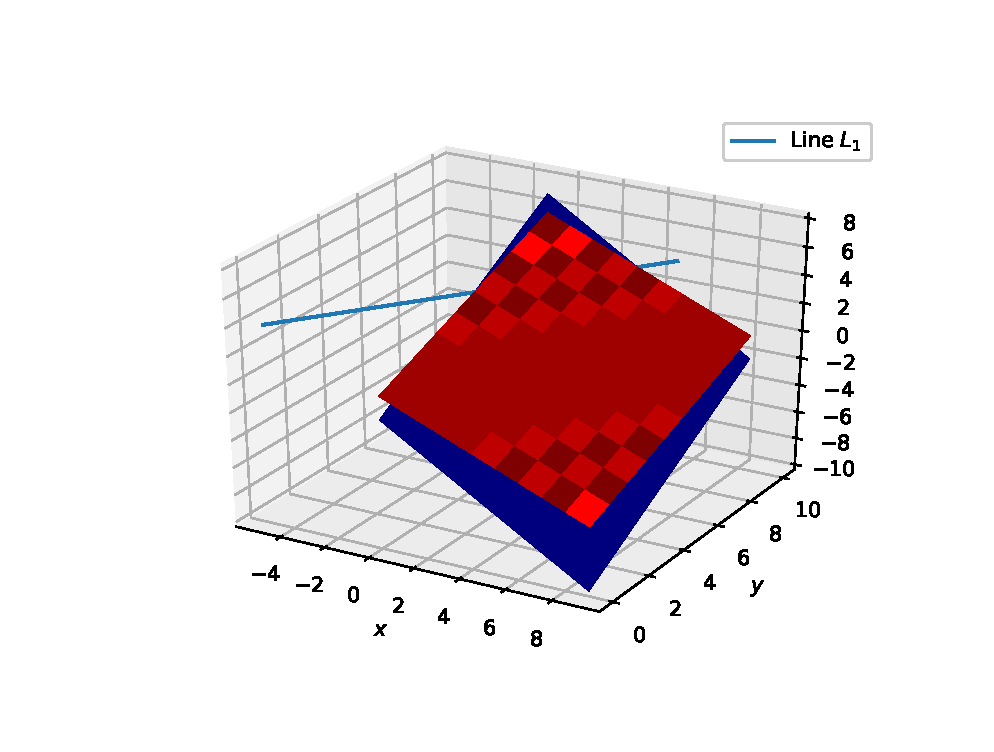
\includegraphics[width=\columnwidth]{./figs/1.1.eps}
\caption{}
\label{fig:1.1}
\end{figure}

\item $L_2$ is the intersection of the planes
\begin{align}
\myvec{1 & 2 & -1}\vec{x} &= 3
\\
\myvec{3 & -1 & 2}\vec{x} &= 1
\end{align}
Show that its equation is
%
\begin{align}
\vec{x} = \frac{1}{7}\myvec{ 5 \\ 8 \\ 0} + \lambda_2 \myvec{ -3 \\ 5 \\ 7}
\label{eq:l2}
\end{align}
\item Plot 
$L_2$.
\\
\solution The following code generates Fig. \ref{fig:1.2}.
\begin{lstlisting}
wget 
https://github.com/gadepall/school/raw/master/linalg/3D/manual/codes/1.2.py
\end{lstlisting}
\begin{figure}[!ht]
\centering
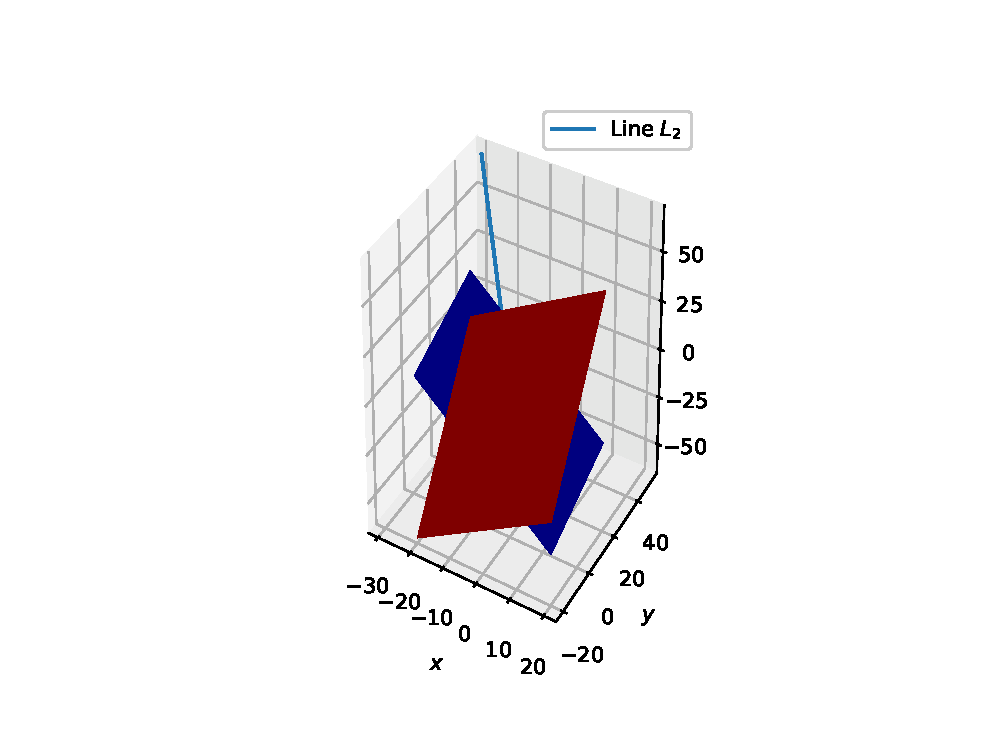
\includegraphics[width=\columnwidth]{./figs/1.2.eps}
\caption{}
\label{fig:1.2}
\end{figure}

\item Do $L_1$ and $L_2$ intersect? If so, find their point of intersection $P$.
\\
\solution From \eqref{eq:l1},\eqref{eq:l2}, the point of intersection is given by
\begin{align}
\label{eq:l1l2pt}
\vec{x} = \frac{1}{7}\myvec{ 5 \\ 8 \\ 0} + \lambda_2 \myvec{ -3 \\ 5 \\ 7} &= \myvec{ 
-5 \\ 0 \\ 4} + \lambda_1 \myvec{ 1 \\ 1 \\ 0}
\\
\implies 
\myvec{1 &  3 \\ 1 & -5 \\ 0 & -7}\vec{\Lambda} &= \frac{1}{7}\myvec{40 \\ 8 \\ -28}
\end{align}
This matrix equation can be solved as
\begin{align}
\myvec{1 &  3 & \frac{40}{7}\\ 1 & -5 &\frac{8}{7}\\ 0 & -7 & -4} &\leftrightarrow \myvec{8 &  0 & 
\frac{224}{7}\\ 0 & 1 &\frac{4}{7}\\ 0 & 1 & \frac{4}{7} }
\\
\leftrightarrow \myvec{1 &  0 & 
4\\ 0 & 1 &\frac{4}{7} } &\implies \vec{\Lambda} = \myvec{4\\\frac{4}{7}}
\end{align}
%
Substituting $\lambda_1 = 4$ in \eqref{eq:l1l2pt}
\begin{align}
\vec{x} = \myvec{4 \\ 4 \\ 0} + \myvec{-5 \\ 0 \\ 4} = \myvec{-1\\ 4\\ 4}
\end{align}
\item Plot $P$.
\\
\solution The following code generates Fig. \ref{fig:1.3}.
\begin{lstlisting}
wget 
https://github.com/gadepall/school/raw/master/linalg/3D/manual/codes/1.3.py
\end{lstlisting}
\begin{figure}[!ht]
\centering
\includegraphics[width=\columnwidth]{./figs/1.3.eps}
\caption{}
\label{fig:1.3}
\end{figure}
\end{enumerate}
\section{Normal to a Plane}
\begin{enumerate}[label=\thesection.\arabic*
,ref=\thesection.\theenumi]
\item The cross product of $\vec{a},\vec{b}$ is defined as
\begin{equation}
\label{eq:cross}
\vec{a}\times \vec{b} = \myvec{0 & -a_3 & a_2 \\ a_3 & 0 & -a_1 \\ -a_2 & a_1 & 0}\myvec{b_1 \\ b_2 \\ b_3}
\end{equation}
From \eqref{eq:l1}, \eqref{eq:l2}, the direction vectors of $L_1$ and $L_2$ are
\begin{equation}
\myvec{1 \\ 1 \\ 0} \text{ and } \myvec{-3 \\ 5 \\ 7}
\end{equation}
respectively. Find the direction vector of the normal to the plane spanned by $L_1$ and $L_2$.
\\
\solution The desired vector is obtained as
\begin{align}
\myvec{1 \\ 1 \\ 0} \times \myvec{-3 \\ 5 \\ 7} = 
 \myvec{0 & 0 & 1 \\ 0 & 0 & -1 \\ -1 & 1 & 0}\myvec{-3 \\ 5 \\ 7}
= \myvec{7 \\ -7 \\ 8} = \vec{n}
\end{align}
\item Summarize all the above computations through a plot 
\\
\solution The following code generates Fig. \ref{fig:2.1}.
\begin{lstlisting}
wget 
https://github.com/gadepall/school/raw/master/linalg/3D/manual/codes/2.1.py
\end{lstlisting}
\begin{figure}[!ht]
\centering
\includegraphics[width=\columnwidth]{./figs/2.1.eps}
\caption{}
\label{fig:2.1}
\end{figure}
\item Find the equation of the plane spanned by $L_1$ and $L_2$.
\\
\solution Let $\vec{x}_0$ be the intersection of $L_1$ and $L_2$.  Then the equation of the plane is
\begin{align}
\brak{\vec{x}-\vec{x}_0}^T\vec{n} &= 0
\\
\implies \vec{x}^T\vec{n} &= \vec{x}_0^T\vec{n}
\\
\implies \vec{x}^T\myvec{7 \\ -7 \\ 8} &= \myvec{-1 & 4 & 4}\myvec{7 \\ -7 \\ 8} =  -3
\end{align}
\item Summarize  the above through a plot. 
\\
\solution The following code generates Fig. \ref{fig:2.2}.
\begin{lstlisting}
wget 
https://github.com/gadepall/school/raw/master/linalg/3D/manual/codes/2.2.py
\end{lstlisting}
\begin{figure}[!ht]
\centering
\includegraphics[width=\columnwidth]{./figs/2.2.eps}
\caption{}
\label{fig:2.2}
\end{figure}
\item
Find the distance of the origin from the plane containing the lines $L_1$ and $L_2$.
\\
\solution The distance from the origin to the plane is given by
\begin{equation}
\frac{\abs{\vec{x}_0^T\vec{n}}}{\norm{n}} = \frac{1}{3\sqrt{2}}
\end{equation}
\end{enumerate}
\section{Projection on a Plane}
\begin{enumerate}[label=\thesection.\arabic*
,ref=\thesection.\theenumi]
%
\item Find the equation of the line $L$ joining the points 
\begin{align}
\vec{A}=\myvec{5 & -1 &4}^T
\\
\vec{B}=\myvec{4 & -1 & 3}^T
\end{align}
\solution The desired equation is
\begin{align}
\vec{x} &= \vec{B} + \lambda\brak{\vec{A}-\vec{B}}
\\
&= \myvec{4 \\ -1 \\ 3} + \lambda \myvec{1 \\ 0 \\ 1}
\label{eq:Lproj}
\end{align}
\item Plot the above line. 
\\
\solution The following code generates Fig. \ref{fig:3.1}.
\begin{lstlisting}
wget 
https://github.com/gadepall/school/raw/master/linalg/3D/manual/codes/3.1.py
\end{lstlisting}
\begin{figure}[!ht]
\centering
\includegraphics[width=\columnwidth]{./figs/3.1.eps}
\caption{}
\label{fig:3.1}
\end{figure}
\item Find the intersection of $L$ and the plane $P$ given by
\begin{equation}
\myvec{1 & 1 & 1}\vec{x} = 7
\label{eq:Pproj}
\end{equation}
\\
\solution From \eqref{eq:Lproj} and \eqref{eq:Pproj},
\begin{align}
 \myvec{1 & 1 & 1}\myvec{4 \\ -1 \\ 3} + \lambda \myvec{1 & 1 & 1}
\myvec{1 \\ 0 \\ 1} &= 7
\\
\implies 6 + 2\lambda &= 7
\\
\implies \lambda &= \frac{1}{2}
\end{align}
%
Substituting in \eqref{eq:Lproj},
\begin{equation}
\vec{x} = \frac{1}{2}\myvec{9 & -1 & 7}
\end{equation}
\item Sketch the line, plane and the point of intersection.
\\
\solution The following code generates Fig. \ref{fig:3.2}.
\begin{lstlisting}
wget 
https://github.com/gadepall/school/raw/master/linalg/3D/manual/codes/3.2.py
\end{lstlisting}
\begin{figure}[!ht]
\centering
\includegraphics[width=\columnwidth]{./figs/3.2.eps}
\caption{}
\label{fig:3.2}
\end{figure}
\item Find $\vec{C} \in P$  such that $AC \perp P$.  
\\
\solution From \eqref{eq:Pproj}, the direction vector of $AC$ is $\myvec{1 & 1 & 1}^T$.  Hence, the equation of 
$AC$ is
\begin{equation}
\vec{x} = \myvec{5 \\ -1 \\ 4} + \lambda_1  \myvec{1 \\ 1 \\ 1}
\end{equation}
Substituting in \eqref{eq:Pproj}
\begin{align}
 \myvec{1 & 1 & 1}\myvec{5 \\ -1 \\ 4} + \lambda \myvec{1 & 1 & 1}
\myvec{1 \\ 1 \\ 1} &= 7
\\
\implies 8 + 3\lambda_1 &= 7
\\
\implies \lambda_1 &= -\frac{1}{3}
\end{align}
Thus,
\begin{align}
\vec{C} = \frac{1}{3}\myvec{14 \\ -4 \\ 11}
\end{align}
%\item Summarize the above through a plot.
%\\
%\solution The following code generates Fig. \ref{fig:3.3}.
%\begin{lstlisting}
%wget 
%https://github.com/gadepall/school/raw/master/linalg/3D/manual/codes/3.3.py
%\end{lstlisting}
%\begin{figure}[!ht]
%\centering
%\includegraphics[width=\columnwidth]{./figs/3.3.eps}
%\caption{}
%\label{fig:3.3}
%\end{figure}
\item Show that if $BD \perp P$  such that $\vec{D} \in P$,
\begin{equation}
\vec{D} = \frac{1}{3}\myvec{13 \\ -2 \\ 10}
\end{equation}
%
\item Find the projection of $AB$ on the plane $P$.
\\
\solution The projection is given by
\begin{align}
CD = \norm{\vec{C}-\vec{D}} = \sqrt{\frac{2}{3}}
%\label{eq:homog}
\end{align}
\end{enumerate}
\section{Coplanar vectors}
\begin{enumerate}[label=\thesection.\arabic*
,ref=\thesection.\theenumi]
\item If $\vec{u}, \vec{A}, \vec{B}$ are coplanar, show that
\begin{equation}
\vec{u}^T\brak{\vec{A}\times \vec{B}} = 0
\label{eq:coplanar}
\end{equation}
%
\item Find $\vec{A}\times \vec{B}$ given
\begin{align}
\vec{A}=\myvec{2 & 3 & -1}^T
\\
\vec{B}=\myvec{0 & 1 & 1}^T
\end{align}
\solution From \eqref{eq:cross},
\begin{align}
\vec{A}\times \vec{B} &= \myvec{0 & 1& 3 \\ -1 & 0 & -2 \\ -3 & 2 & 0}\myvec{0 \\ 1 \\ 1}
\\
&= \myvec{4 \\ -2 \\ 2}
\label{eq:last_axb}
\end{align}

\item Let $\vec{u}$ be coplanar with 
%
such that $\vec{u}\perp\vec{A}$and
\begin{equation}
\vec{u}^T\vec{B} = 24.
\label{eq:uB}
\end{equation}
Find $\norm{\vec{u}}^2$.
\\
\solution From \eqref{eq:last_axb} and the given information,
\begin{align}
\vec{u}^T\myvec{4 & -2 & 2} &=0
\\
\vec{u}^T\myvec{2 & 3 & -1} &=0
\\
\vec{u}^T\myvec{0 & 1 & 1} &=24
\\
\implies \myvec{4 & -2 & 2
\\
2 & 3 & -1
\\
0 & 1 & 1
}\vec{u}
&= \myvec{0 \\ 0 \\ 24}
\\
\implies 
\vec{u} &= 4 \myvec{-1 \\ 2 \\ 4}
\\
\implies \norm{\vec{u}}^2 &= 336
\end{align}
\end{enumerate}
\section{Least Squares}
\begin{enumerate}[label=\thesection.\arabic*
,ref=\thesection.\theenumi]
\item Find the equation of the plane $P$
containing the vectors 
%
\begin{align}
\label{eq:least_vecs}
\vec{x}_1 = \myvec{1 \\ 1 \\ 1}
,
\vec{x}_2 = \myvec{0 \\ 1 \\ 2}
\end{align}
%
\item Show that the vector 
\begin{align}
\vec{y} = \myvec{6 \\ 0 \\ 0}
\end{align}
lies outside $P$.
\item Find the point $\vec{w} \in P$ closest to $\vec{y}$.
\item Show that
\begin{align}
\norm{\vec{y}-\vec{X}\vec{w}}^2 &= \norm{\vec{y}}^2 - \vec{w}^T\vec{X}^T\vec{y} 
\\
& \quad - \vec{y}^TA\vec{w}+\vec{w}^T\vec{X}^T\vec{X}\vec{w}
\end{align}
%
\item Assuming $2\times 2$ matrices and $2 \times 1$ vectors, show that
\begin{align}
\frac{\partial}{\partial\vec{w}}\vec{w}^T\vec{X}^T\vec{y} = \frac{\partial}{\partial\vec{w}}\vec{y}^T\vec{X}\vec{w} = 
\vec{y}^T\vec{X}
\end{align}
\item Show that
\begin{align}
\frac{\partial}{\partial\vec{w}}\vec{w}^T\vec{X}^T\vec{X}\vec{w} = 2\vec{w}^T\brak{\vec{X}^T\vec{X}}
\end{align}
\item Show that 
\begin{align}
\hat{\vec{w}} &= \min_{\vec{w}}\norm{\vec{y}-\vec{X}\vec{w}}^2
\\
 &= \brak{\vec{X}^T\vec{X}}^{-1}\vec{X}^T \vec{y}
\label{eq:least_sol}
\end{align}
\item Let 
\begin{align}
\vec{X} = \myvec{\vec{x}_1 & \vec{x}_2}.
\end{align}
from \eqref{eq:least_vecs}.
Verify \eqref{eq:least_sol}.
\end{enumerate}
\section{Linear Algebra: Orthogonality}
\begin{enumerate}[label=\thesection.\arabic*
,ref=\thesection.\theenumi]

\item Let
\begin{align}
L_1: \quad \vec{x} &= \myvec{1 \\ 0 \\ 0} + \lambda_1 \myvec{-1 \\ 2 \\ 2}
\\
L_2: \quad \vec{x} &=  \lambda_1 \myvec{2 \\-1 \\ 2}
\end{align}
%
Given that  $L_3 \perp L_1, L_3 \perp L_2$, find $L_3$.
\\
\solution Let 
\begin{align}
L_3: \quad \vec{x} &= \vec{c}+ \lambda \vec{m}_3
\end{align}
% 
Then
\begin{align}
\myvec{-1 & 2 & 2
\\
2 &-1 & 2}\vec{m}_3 = \vec{0}
\end{align}
%
Row reducing the coefficient matrix,
\begin{align}
\myvec{-1 & 2 & 2
\\
2 &-1 & 2} &\leftrightarrow 
\myvec{1 & -2 & -2
\\
0 &1 & 2} 
\\
\leftrightarrow 
\myvec{1 & 0 & 2
\\
0 &1 & 2} 
& \implies \vec{m}_3 = \myvec{2 \\ 2 \\ -1}
\end{align}
%
Also, $L_1\perp L_2$, but $L_1 \cup L_2 = \phi$. The given information can be summarized as
\begin{align}
\label{eq:12-given1}
L_1: \quad \vec{x} &= \vec{c}_1 + \lambda_1 \vec{m}_1
\\
L_2: \quad \vec{x} &=  \lambda_2 \vec{m}_2
\\
L_3: \quad \vec{x} &= \vec{c}_3 + \lambda \vec{m}_3
\label{eq:12-given3}
\end{align}
%
where
\begin{align}
\label{eq:12-given12}
\vec{c}_1 = \myvec{1 \\ 0 \\ 0}, \vec{m}_1=  \myvec{-1 \\ 2 \\ 2},
\vec{m}_2 = \myvec{2 \\-1 \\ 2}
\end{align}
The objective is to find $\vec{c}_3$.  Since $L_1 \cup L_3 \ne \phi, L_2 \cup L_3 \ne \phi$, from \eqref{eq:12-given1}-\eqref{eq:12-given3},
\begin{align}
\label{eq:12-isect13}
\vec{c}_1 + \lambda_1 \vec{m}_1 &= \vec{c}_3 + \lambda_3 \vec{m}_3
\\
  \lambda_2 \vec{m}_2 &= \vec{c}_3 + \lambda_4 \vec{m}_3
\label{eq:12-isect23}
\end{align}
%
Using the fact that $L_1\perp L_2\perp L_3$, \eqref{eq:12-isect13}-\eqref{eq:12-isect23} can be expressed as
\begin{align}
%\label{eq:12-isect13}
\vec{m}_1^T\vec{c}_1 + \lambda_1 \norm{\vec{m}}_1^2 &= \vec{m}_1^T\vec{c}_3 
\\
\vec{m}_2^T\vec{c}_1  &= \vec{m}_2^T\vec{c}_3 
\\
\vec{m}_3^T\vec{c}_1  &= \vec{m}_3^T\vec{c}_3 + \lambda_3 \norm{\vec{m}_3}^2
\\
0 &= \vec{m}_1^T\vec{c}_3 
\\
  \lambda_2 \norm{\vec{m}_2}^2 &= \vec{m}_2^T\vec{c}_3 
\\
0 &= \vec{m}_3^T\vec{c}_3  + \lambda_4 \norm{\vec{m}_3}^2
%\label{eq:12-isect23}
\end{align}
%
Simplifying the above, 
\begin{align}
 \lambda_1  &= -\frac{\vec{m}_1^T\vec{c}_1}{\norm{\vec{m}}_1^2} = \frac{1}{9}
\\
 \lambda_2  &= \frac{\vec{m}_2^T\vec{c}_1}{\norm{\vec{m}}_2^2} =\frac{2}{9}
\end{align}
%
Substituting in \eqref{eq:12-isect13} and \eqref{eq:12-isect23},
\begin{align}
L_3: \quad \vec{x} &= \frac{2}{9}\myvec{4 \\ 1 \\ 1} + \lambda_3\myvec{2 \\ 2 \\ -1} \text{ or}
\\
L_3: \quad \vec{x} &= \frac{2}{9}\myvec{2 \\-1 \\ 2} + \lambda_3\myvec{2 \\ 2 \\ -1}
\end{align}
%
The key concept in this question is that orthogonality of $L_1$ and $L_2$ doesnot mean that they intersect.  They are skew lines.
\end{enumerate}
%

%\section{Vector Algebra}
%\begin{enumerate}[label=\thesection.\arabic*
%,ref=\thesection.\theenumi]
%
%\item The line 
%\begin{align}
%\Gamma: \vec{x} = \myvec{0 \\ 1} + \lambda \myvec{1 \\ m}
%\label{eq:coord_line}
%\end{align}
%intersects the circle
%\begin{align}
%\Omega: \norm{\vec{x}-\myvec{3 \\ -2}} = 5
%\label{eq:coord_circ}
%\end{align}
%at points $\vec{P}$ and $\vec{Q}$ respectively. The mid point of $PQ$ is 
%$\vec{R}$ such that
%\begin{align}
%\myvec{1 & 0}\vec{R} = -\frac{3}{5}
%\label{eq:coord_mid}
%\end{align}
%%
%Find $m$.
%\\
%\solution Let 
%\begin{align}
%\vec{c} = \myvec{0 \\ 1}, \vec{O} = \myvec{3 \\ -2} \text{ and } \vec{m} = 
%\myvec{1 \\ m}
%\label{eq:coord_defs}
%\end{align}
%%
%The intersection of  \eqref{eq:coord_line} and \eqref{eq:coord_circ} is 
%\begin{align}
%\norm{\vec{c}+\lambda\vec{m} -\vec{O}}^2 = 25
%\end{align}
%\begin{multline}
%\label{eq:coord_quad}
%\implies \lambda^2 \norm{\vec{m}}^2+ 2\lambda\vec{m}^{T}\brak{\vec{c} 
%-\vec{O}}
%\\
%+\norm{\vec{c} -\vec{O}}^2-25 = 0
%\end{multline}
%%
%Since $\vec{P}, \vec{Q}$ lie on $\Gamma$,
%\begin{align}
%\vec{P} &= \vec{c}+\lambda_1\vec{m} 
%\\
%\vec{Q} &= \vec{c}+\lambda_2\vec{m} 
%\\
%\implies \frac{\vec{P}+\vec{Q}}{2} &= \vec{c} + 
%\frac{\lambda_1+\lambda_2}{2}\vec{m} 
%\\
%\implies \myvec{1 & 0}\frac{\vec{P}+\vec{Q}}{2} &= \myvec{1 & 0}\vec{c}
%\nonumber \\
%& \,+ \frac{\lambda_1+\lambda_2}{2}\myvec{1 & 0}\vec{m} 
%\\
%&= \myvec{1 & 0}\vec{c} -
%\frac{\vec{m}^{T}\brak{\vec{c} -\vec{O}}}{\norm{\vec{m}}^2}
%\end{align}
%using the sum of roots in \eqref{eq:coord_quad}.  From 
%\eqref{eq:coord_mid} and \eqref{eq:coord_defs},
%\begin{align}
%-\myvec{1 & m}\myvec{-3\\3}= -\frac{3}{5}\brak{1+m^2}
%\\
%\implies m^2 -5m + 6 = 0
%\\
%\implies m = 2 \text{ or } 3
%\end{align}
%From \eqref{eq:coord_quad}, 
%\begin{multline}
%\lambda = \frac{-\vec{m}^{T}\brak{\vec{c} -\vec{O}}}{{\norm{\vec{m}}^2}}
%\\
%\pm \frac{\sqrt{\brak{\vec{m}^{T}\brak{\vec{c} -\vec{O}}}^2
%-\norm{\vec{c} -\vec{O}}^2+25}}{\norm{\vec{m}}^2}
%\end{multline}
%Fig. \ref{fig:2019_3} summarizes the solution for $m = 2$.
%
%%\renewcommand\thefigure{\theenumi}
%
%\begin{figure}
%\centering
%\includegraphics[width=\columnwidth]{./figs/2019_3.eps}
%\caption{}
%\label{fig:2019_3}
%\end{figure}
%\end{enumerate}

\section{Linear Algebra: Area of a Triangle}
\begin{enumerate}[label=\thesection.\arabic*
,ref=\thesection.\theenumi]

\item Let  the lines
\begin{align}
L_1: \vec{x} &=  \lambda_1 \vec{a}
\\
L_2: \vec{x} &=  \lambda_2 \vec{b}
\\
L_3: \vec{x} &=  \lambda_3 \vec{c}
\end{align}
%
intersect the plane 
\begin{align}
P: \vec{n}^{T}\vec{x} = c
\end{align}
%
at the points $\vec{A},\vec{B}$ and $\vec{C}$ respectively. 
Find $\lambda_1,\lambda_2$ and $\lambda_3$.
\\
\solution 
From the given information, $\vec{A} \in P, L_1$. $\because \vec{A} = \lambda_1 \vec{a}$,
\begin{align}
\label{eq:18_lambda}
\lambda_1\vec{n}^T\vec{a} = c \implies \lambda_1 =  \frac{c}{\vec{n}^T\vec{a}}
\end{align}
%
Similarly, $\lambda_2$ and $\lambda_3$ are obtained.
\item Find the area $\Delta$ of $\triangle ABC$  
\\
\solution 
\begin{align}
\Delta &= \norm{\frac{1}{2}\brak{\vec{A}-\vec{B}}\times\brak{\vec{A}-\vec{C}}}
\nonumber \\
&= \frac{1}{2}\norm{\brak{\lambda_1\vec{a}-\lambda_2\vec{b}}\times\brak{\lambda_1\vec{a}-\lambda_3\vec{c}}}
\nonumber \\
&= \frac{1}{2}\Vert\lambda_1\lambda_2\brak{\vec{a}\times \vec{b}}+\lambda_2\lambda_3\brak{\vec{b}\times \vec{c}}
\nonumber \\ 
&\quad +\lambda_1\lambda_3\brak{\vec{c}\times\vec{a}}\Vert
\end{align}
\item Find  $\brak{6\Delta}^2$ given 
\begin{align}
 \vec{a} &= \myvec{1 \\ 0\\ 0},
 \vec{b} = \myvec{1 \\ 1\\ 0},
 \vec{c} = \myvec{1 \\ 1\\ 1},
\\
\vec{n} &= \myvec{1 & 1 & 1}, c= 1
\end{align}
%
\solution 
\begin{align}
\label{eq:18_cross}
\vec{a}\times \vec{b} &= \myvec{0 & -a_3 & a_2 \\ a_3 & 0 & -a_1 \\ -a_2 & a_1 & 0}\myvec{b_1 \\ b_2 \\ b_3}
\nonumber \\
&= \myvec{0 & 0 & 0 \\ 0 & 0 & -1 \\ 0 & 1 & 0}\myvec{1 \\ 1 \\ 0}
=\myvec{0 \\ 0 \\ 1}
\\
\vec{b}\times \vec{c} &= \myvec{0 & 0 & 1 \\ 0 & 0 & -1 \\ -1 & 1 & 0}\myvec{1 \\ 1 \\ 1}
%\nonumber \\
= \myvec{1 \\ -1 \\ 0}
\\
\vec{c}\times \vec{a} &= \myvec{0 & -1 & 1 \\ 1 & 0 & -1 \\ -1 & 1 & 0}\myvec{1 \\ 0 \\ 0}
%\nonumber \\
= \myvec{0 \\ 1 \\ -1}
\end{align}
%
Using \eqref{eq:18_lambda},
\begin{align}
\lambda_1=1, \lambda_2 = \frac{1}{2}, \lambda_3 = \frac{1}{3}
\end{align}
Thus,
\begin{align}
\Delta &= \frac{1}{2}\norm{\frac{1}{2}\myvec{0 \\ 0 \\ 1}+\frac{1}{6}\myvec{1 \\ -1 \\ 0}+\frac{1}{3}\myvec{0 \\ 1 \\ -1}}
\\
&= \frac{1}{12}\norm{\myvec{1 \\ 1 \\ 1}} = \frac{\sqrt{3}}{12}
\end{align}
%
Hence,
\begin{align}
\brak{6 \Delta}^2 = \frac{3}{2}
\end{align}
\end{enumerate}
\section{Linear Algebra: Linear Dependence}
\begin{enumerate}[label=\thesection.\arabic*
,ref=\thesection.\theenumi]
\item Let
\begin{align}
\label{eq:qp2-8-l_1}
L_1: \quad \vec{r} = \lambda_1 \myvec{1\\0\\0}
\\
\label{eq:qp2-8-l_2}
L_2: \quad \vec{r} = \myvec{0\\0\\1}+\lambda_2 \myvec{0\\1\\0}
\\
L_3: \quad \vec{r} =  \myvec{1\\1\\0}+\lambda_3 \myvec{0\\0\\1}
\label{eq:qp2-8-l_3}
\end{align}
%
Let $\vec{P}\in L_1, \vec{Q}\in L_2, \vec{R}\in L_3$. Given that   $\vec{P},\vec{Q},\vec{R}$ are collinear,
If $\vec{P},\vec{Q},\vec{R}$ are collinear, find $\vec{Q}$.
\\
\solution 
\begin{align}
\frac{PQ}{QR} &= k,
\\
\brak{k+1}\vec{Q} &= k\vec{P}+ \vec{R},
\label{eq:qp2-8-coll}
\end{align}
From \eqref{eq:qp2-8-l_1}, \eqref{eq:qp2-8-l_2} and \eqref{eq:qp2-8-l_3},
\begin{multline}
k \lambda_1 \myvec{1\\0\\0}
+\myvec{1\\1\\0}+\lambda_3 \myvec{0\\0\\1}
\\
=
\brak{k+1} \myvec{0\\0\\1}+\brak{k+1}\lambda_2 \myvec{0\\1\\0}
\end{multline}
%
which can be expressed as
\begin{align}
\myvec{k & 0 & 0
\\
0 & -\brak{k+1} & 0
\\
0 & 0 & 1
}
\myvec{\lambda_1\\\lambda_2\\ \lambda_3}
=\myvec{-1 \\ -1 \\ k+1}
\end{align}
%
Thus,
\begin{align}
\vec{Q} = \myvec{0 \\\frac{1}{k+1} \\1}
\end{align}
\item Verify if  $\vec{Q}$ can be 

\begin{enumerate}
\begin{multicols}{2}
\setlength\itemsep{1em}
\item $\myvec{0\\-\frac{1}{2} \\ 1}$
\item $\myvec{0\\ 0\\1}$
\item $\myvec{0\\ \frac{1}{2} \\1}$
\item $\myvec{0\\1 \\1}$
\end{multicols}
\end{enumerate}
\end{enumerate}
\section{Linear Algebra: Projection}
\begin{enumerate}[label=\thesection.\arabic*
,ref=\thesection.\theenumi]
\item Show that the projection of $\vec{x}$ on $\vec{y}$ is
\begin{align}
\label{eq:2019_qp2_14_proj}
\frac{\vec{x}^T\vec{y}}{\norm{\vec{y}}^2}\vec{y}
\end{align}
\item Given 
\begin{align}
\label{eq:2019_qp2_14_cab}
\vec{c} = \alpha \vec{a}+\beta\vec{b},
\end{align}
show that 
\begin{align}
\brak{\vec{c}-\brak{\vec{a}\times\vec{b}}}^{T}\vec{c} = \norm{\vec{c}}^2
\end{align}
%
%
\item Find 
\begin{align}
\label{eq:2019_qp2_14_prob}
\min_{\vec{u}} \norm{\vec{c}}^2
\\
s.t \quad 
\norm{\text{proj}_{\vec{a}+\vec{b}}\vec{c}} = 3\sqrt{2}
\label{eq:2019_qp2_14_const}
\end{align}
%
by using the fact that 
\begin{align}
\vec{c}&=\vec{P}\vec{u}
\\
\vec{a}+\vec{b} &= \vec{P}\vec{1}
\end{align}
%
where 
\begin{align}
\vec{P} &= \myvec{\vec{a} &\vec{b}}
\\
\vec{u} &= \myvec{\alpha \\ \beta}
\\
\vec{1} &= \myvec{1 \\ 1}
\end{align}
\end{enumerate}

\end{document}
